\documentclass[a4paper, 12pt]{article}

\usepackage[english,russian]{babel}
\usepackage[left=2cm, top=2cm, right=2cm, bottom=2.5cm]{geometry}
\usepackage{amssymb}
\usepackage{amsmath}
\usepackage{graphicx}
\usepackage[tableposition=top,singlelinecheck=false]{caption}
\usepackage{tabularx}

\title{Изотермическое растяжение резины. Изменение энтропии. Зависимость растяжения от силы. Оценка модуля Юнга.}
\author{Леонид Пилюгин, Б02-212}

\DeclareMathOperator{\const}{const}

\begin{document}
    \maketitle

    \section{Параметры установки}
    \begin{enumerate}
        \item Длина нерастянутой резинки $l_0=11\pm 0{,}1\,\text{см}$
        \item Ширина нерастянутой резинки $d_0=12\pm 0{,}5\,\text{мм}$
        \item Толщина нерастянутой резинки $h_0=1{,}75\pm 0{,}05\,\text{мм}$
        \item $g=9{,}8155\,\text{кг}/\text{м}\cdot\text{с}^2$
    \end{enumerate}

    \section{Теория}

    Внутренняя жнергия резины определяется только температурой, а её работа равна
    \[\delta A = -fdl\]

    Тогда при изотермическом растяжении
    \[\delta Q = TdS=-fdl\]
    \[f=-\left(\frac{\partial Q}{\partial l}\right)_T =
    -T\left(\frac{\partial S}{\partial l}\right)_T =
    T\left(\frac{\partial f}{\partial T}\right)_l\]

    Это возможно только если сила прямо пропорциональна температуре:
    \[f(T, l) = \frac{T}{T_0}\overline{f}\left(\frac{l}{l_0}\right)\]

    Вид функции $\overline{f}$ определятеся эмперическими и полуэмперическими моделями.
    В наиболее удачной
    \[\Delta S = -\const\cdot\left(\lambda^2+\frac{2}{\lambda}\right)\]
    \[f(\lambda)=\frac{1}{3}s_0E\left(\lambda-\frac{1}{\lambda^2}\right)\]

    \section{Измеряемые данные}

    \subsection{Зависимость $f(\lambda)$}
    \begin{enumerate}
        \item Наклон $k=11{,}7\pm 0{,}9\,\text{Н}$
        \item Модуль Юнга $E=\frac{k}{d_0h_0}=0{,}56\pm 0{,}08\,\text{МПа}$
    \end{enumerate}

    \subsection{Зависимость $f(\lambda-1/\lambda^2)$}
    \begin{enumerate}
        \item Наклон $k=8{,}5\pm 0{,}9\,\text{Н}$
        \item Модуль Юнга $E=3\frac{k}{d_0h_0}=1{,}2\pm 0{,}2\,\text{МПа}$
    \end{enumerate}

    \begin{table}[ht!]
        \caption{Измеряемые данные}
        \begin{tabular}{|l|l|}
        \hline
        $L,\pm0{,}05\text{см}$ & $m,\,\text{г}$ \\ \hline
        $14{,}8$               & $287{,}8$    \\ \hline
        $15{,}2$               & $389{,}6$    \\ \hline
        $15{,}7$               & $466{,}0$    \\ \hline
        $16{,}2$               & $567{,}8$    \\ \hline
        $16{,}8$               & $744{,}6$    \\ \hline
        $17{,}1$               & $813{,}0$    \\ \hline
        $17{,}6$               & $846{,}4$    \\ \hline
        $18{,}3$               & $919{,}4$    \\ \hline
        $19{,}0$               & $989{,}7$    \\ \hline
        $19{,}4$               & $1021{,}2$   \\ \hline
        $20{,}7$               & $1122{,}6$   \\ \hline
        $22{,}0$               & $1224{,}4$   \\ \hline
        $23{,}6$               & $1325{,}4$   \\ \hline
        $24{,}8$               & $1427{,}2$   \\ \hline
        \end{tabular}
    \end{table}

    \begin{figure}
        \centering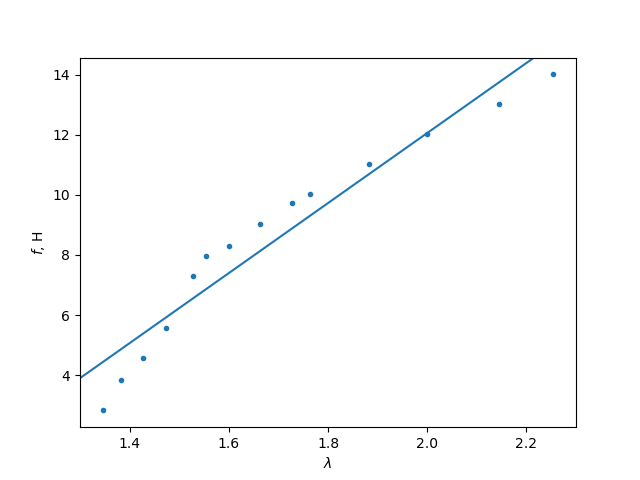
\includegraphics[width=0.8\linewidth]{img/lol.png}
        \caption{Зависимость $f(\lambda)$}
    \end{figure}

    \begin{figure}
        \centering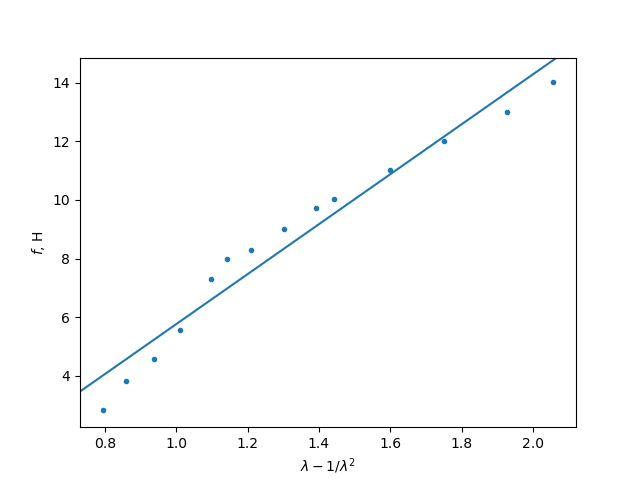
\includegraphics[width=0.8\linewidth]{img/kek.png}
        \caption{Зависимость $f(\lambda-1/\lambda^2)$}
    \end{figure}

\end{document}